\documentclass[a4paper,11pt]{article}
\usepackage[utf8]{inputenc}
\usepackage[pdftex]{graphicx}
\usepackage{pdfpages}
\usepackage{makeidx}
\usepackage[english]{babel}
\usepackage [autostyle, english = american]{csquotes}
\usepackage{amsmath}
\usepackage{xcolor}
\usepackage{listings}
\usepackage{caption,subcaption}
%\usepackage{subfigure}
\usepackage{geometry}
\usepackage{adjustbox}
\usepackage{calc}
\usepackage{ifthen}
\usepackage{listings}
\usepackage{hyperref}
\usepackage[square,sort,comma,numbers]{natbib}
\usepackage{cleveref}
\usepackage[section,cachedir=build,newfloat]{minted}
\usepackage{chngcntr}


\definecolor{mintedbackground}{rgb}{0,0,0}


\usemintedstyle{tango}
\newenvironment{code}{\captionsetup{type=listing}}{}
\SetupFloatingEnvironment{listing}{name=Source Code}
\captionsetup[subfigure]{subrefformat=simple,labelformat=simple}

\renewcommand{\thelisting}{\arabic{listing}}
\renewcommand\thesubfigure{(\alph{subfigure})}

\bibliographystyle{abbrvnat}

\geometry{
 a4paper,
 total={170mm,257mm},
 left=20mm,
 top=20mm,
}
 
\hypersetup{
    colorlinks,
    citecolor=black,
    filecolor=black,
    linkcolor=black,
     urlcolor=black
}
 
\graphicspath{ {images/} }


\newmintedfile[pycode]{python3}{
frame=lines,
framesep=2mm,
fontsize=\footnotesize,
showtabs =false,
autogobble=true,
breaklines=true,
}

\title{Assignment 1 \\ Introduction to Information Retrieval \\ CS734/834}
\author{John Berlin}
\date{\today}
\renewcommand\thesection{Q.\arabic{section}}
\renewcommand\thesubsection{\thesection}

\begin{document}
\maketitle
\newpage
\section{Question 1.2}
\begin{verbatim}
Site search is another common application of search engines. In this case,
search is restricted to the web pages at a given website. 
Compare site search to web search, vertical search, and enterprise search
\end{verbatim}
\subsection{Answer}
% trim={<left> <lower> <right> <upper>}
To compare the four searches I performed the first three using Google and base query ``async redux". 
The search results shown are limited to the first three in order to have presentable figures.
For the site search I used the site \textit{github.com} as the context for the base query is developing web pages in the React.js ecosystem.
As seen in figure \hyperref[fig:ssearch]{\ref{fig:ssearch}} the results are for libraries that do async actions in redux. The first two is from the redux library itself whereas the third is from a library that enhances that functionality.  \newline

The web searches top three results figure \hyperref[fig:wwwearch]{\ref{fig:wwwsearch}}, featured two results from the online documentation of the library itself and one code example which the first result of the site search.  These results were as expected as the query was missing the context given to search engine through the ``site:github.com" as is done in site search. The context is key when comparing site search to web search as it effects the precision of these queries rather than recall. For example, I made this exact query recently when looking into how to better handle the async problems faced by WAIL\footnotemark \footnotetext{https://github.com/N0taN3rd/wail} which is using flux (the predecessor to redux). I performed the web search first as I wanted to see in the documentation on how redux handled async operations rather than diving into the code bases of the libraries themselves. Google understood the likely hood of this happening for the base query and was precise in its top three results given the lack of context which is present in the site search.
\newline 

Vertical search is done when only results of a certain type are desired which is another contextual based query. The results of this search, using Google Videos figure \hyperref[fig:vsearch]{\ref{fig:vsearch}}, in comparison to the site search can be described as combination of the web search and the site site search. The first two results of this query are a combination of all three results from the web search plus the first and second of the site search. The last result of the vertical search features content from the third result from the site search. 
\newline 

In order to compare enterprise search to site search I will use two examples: the first will be the classical example using my personal computers file search. The second will be using more targeted search on my personal computer within the context of the previous two comparisons. As I do not have a large corporate intranet to search I use \emph{Desktop Search} in this example. Desktop search, as defined in our book, is the personal version of enterprise search \citep[pp. 3]{CroftMetzlerStrohman200902}. I felt this is a correct substitution because the previous two comparisons used examples about how I personally used the them for WAIL. Furthermore if a team of developers was looking to find out where on their computers which libraries are currently being used for async operations figure \hyperref[fig:cdeSearch]{\ref{fig:cdeSearch}} and then where in the repository is the functionality implemented figure \hyperref[fig:tdeSearch]{\ref{fig:tdeSearch}}.

Enterprise Search (\emph{Desktop Search}) returned results that had the search term in them not necessarily the most relevant figure \hyperref[fig:cdeSearch]{\ref{fig:cdeSearch}}. The search term async can be found in directory names as well as many duplicates. The duplicates in these results are a product of the search being done on the file system where duplicates are acceptable. Unlike site search which returned unique results where duplicates are not as common. Whereas if you were to use the Linux utility \emph{grep}, you can perform the same kind of query but limited to lines contained in the files in a specific part of the file system figure \hyperref[fig:tdeSearch]{\ref{fig:tdeSearch}}, much like site search. It is clear to see that enterprise search is a broader type of search yet is done a specific site(file system).

\begin{figure}[h]
\adjustbox{trim={0} {0.5\height} {0} {0},clip}%
  {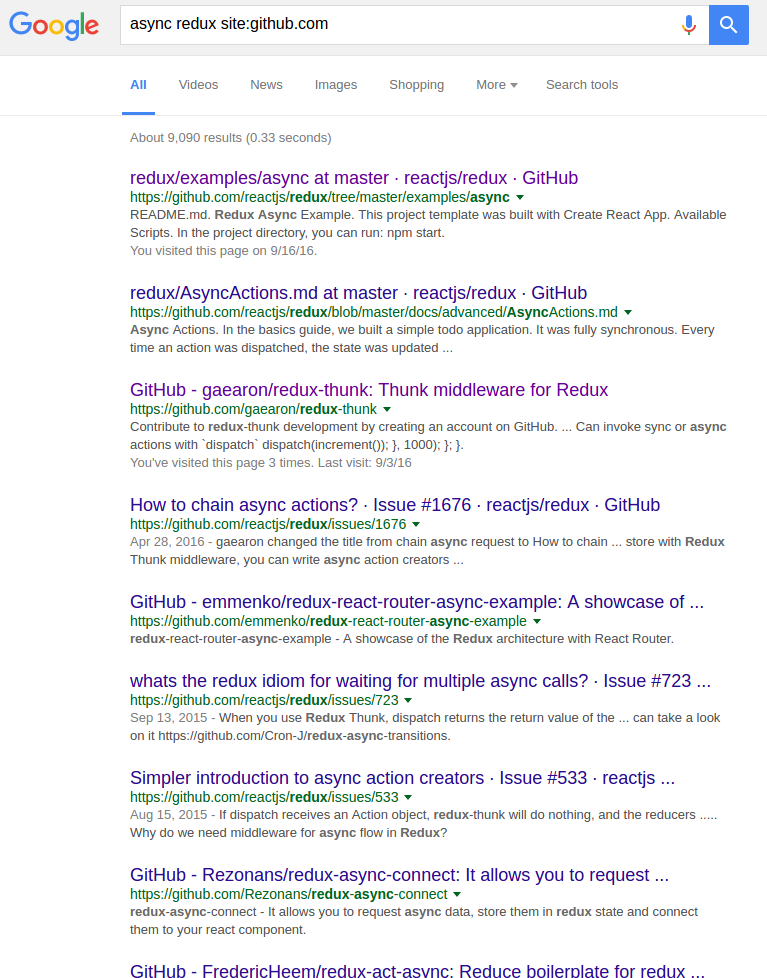
\includegraphics[scale=0.5]{googleSiteSearch.png}}
\caption{Site Search}
\label{fig:ssearch}
\end{figure}
\begin{figure}[h]
\adjustbox{trim={0} {0.5\height} {0} {0},clip}%
  {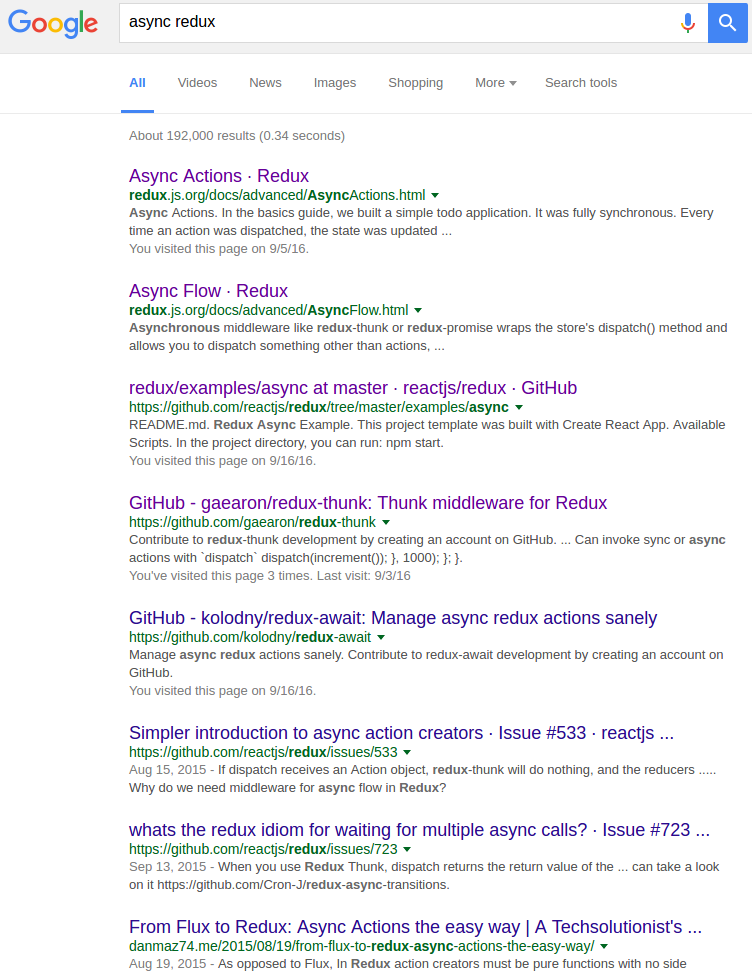
\includegraphics[scale=0.5]{googleWWWSearch.png}}
\caption{Web Search}
\label{fig:wwwsearch}
\end{figure}
\begin{figure}[h]
\adjustbox{trim={0} {0.5\height} {0} {0},clip}%
  {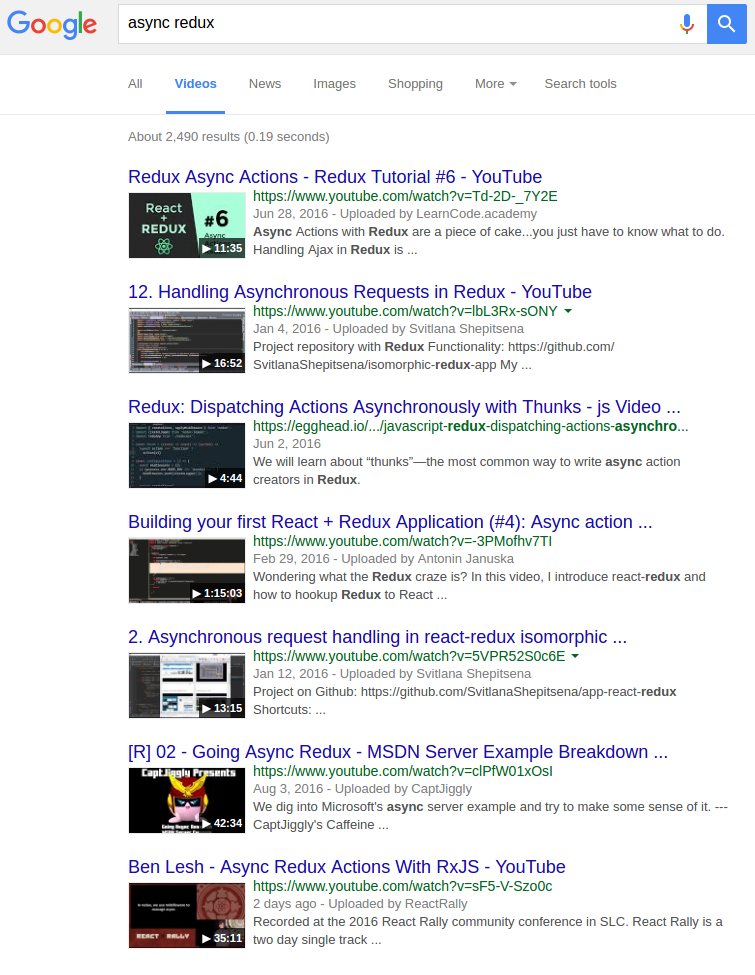
\includegraphics[scale=0.5]{googleVerticalSearch.png}}
\caption{Vertical Search}
\label{fig:vsearch}
\end{figure}
\begin{figure}[h]
\begin{subfigure}{0.45\textwidth}
        \adjustbox{trim={0} {0.5\height} {0.3\width} {0},clip}
		  {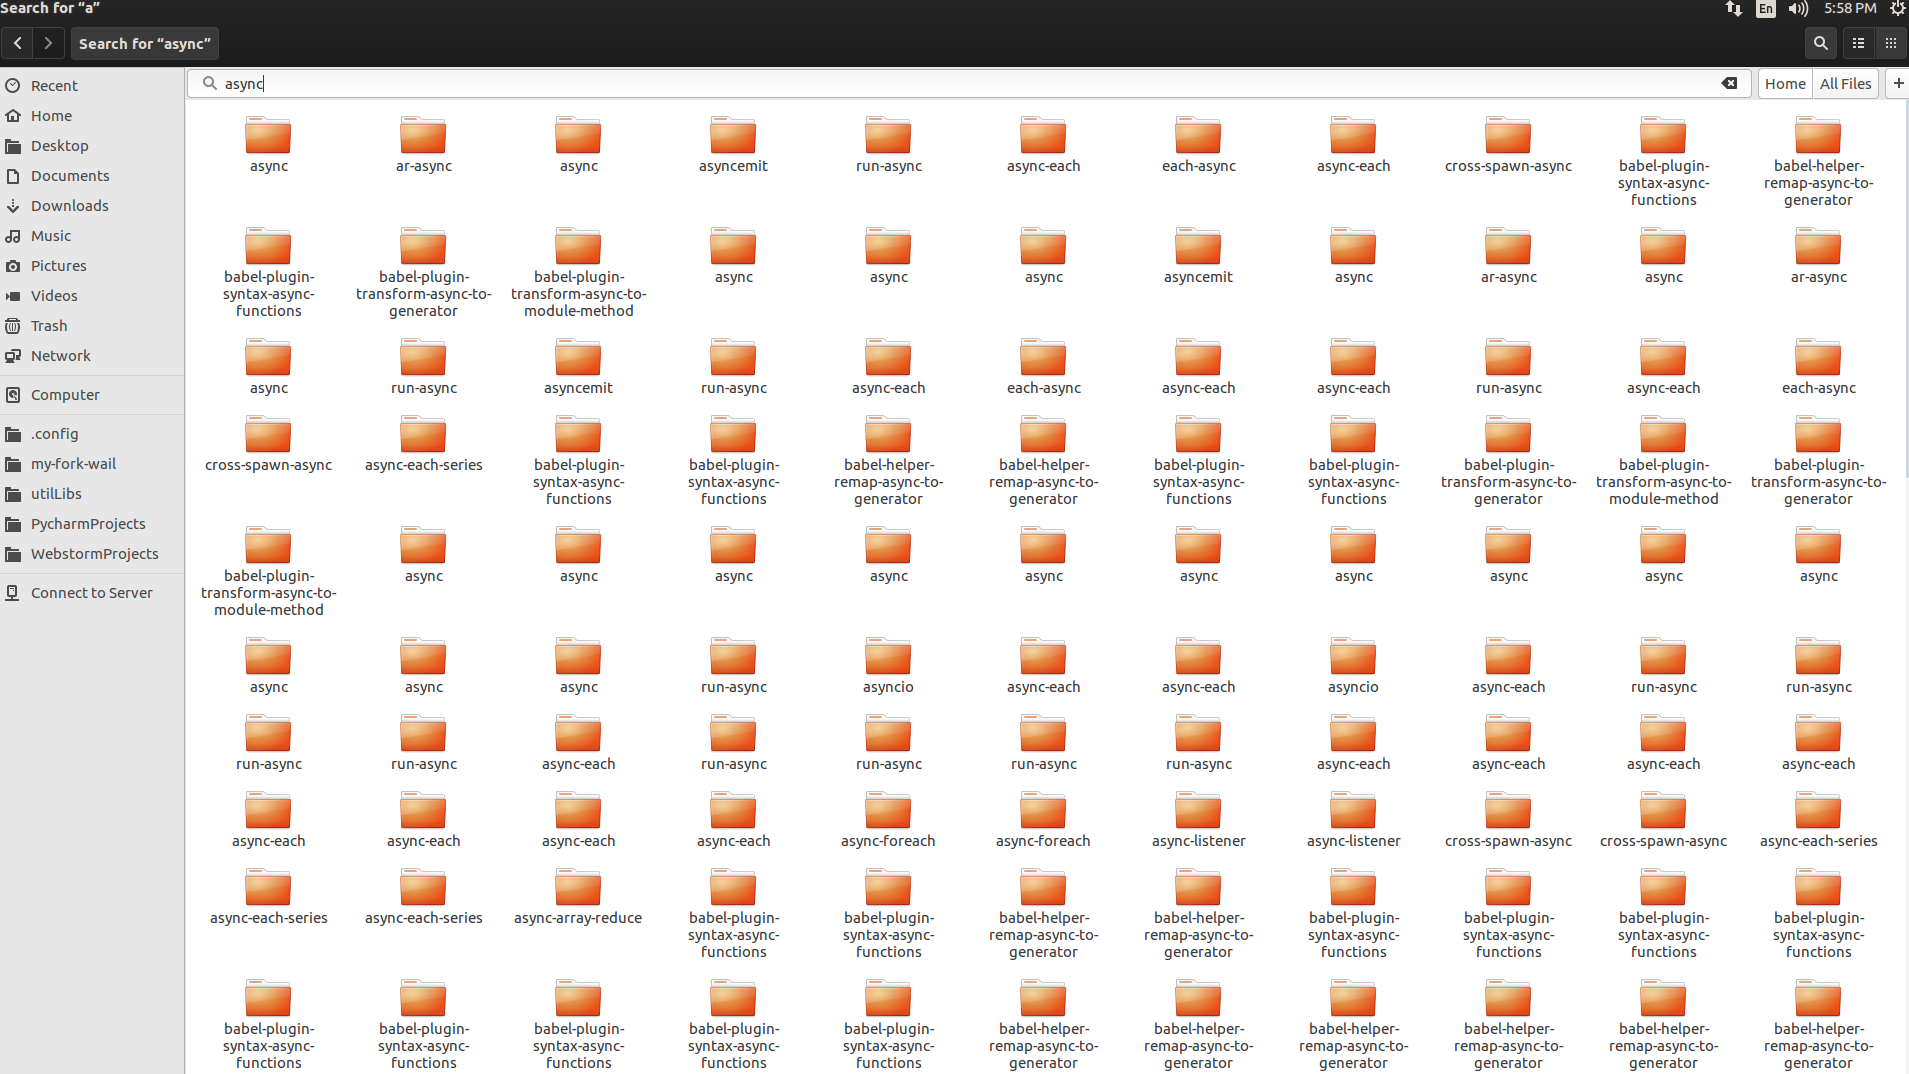
\includegraphics[scale=0.3]{eSearch2.png}}
          \caption{Classic}
          \label{fig:cdeSearch}
      \end{subfigure}
      \vfill
      \begin{subfigure}{0.45\textwidth}
        \adjustbox{trim={0} {0.5\height} {0} {0},clip}
  {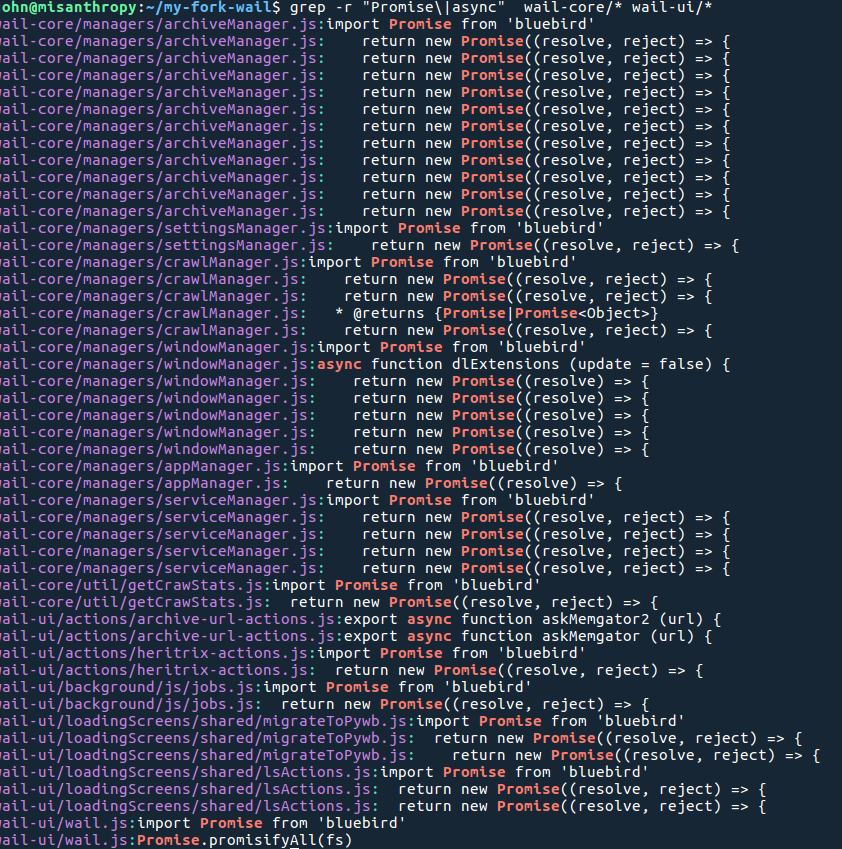
\includegraphics[scale=0.5]{eSearch.png}}   
    \caption{Targeted}
          \label{fig:tdeSearch}
      \end{subfigure}
      \caption{Enterprise Search}
  \label{fig:esearch}
\end{figure}
\newpage
\clearpage
\section{Question 3.7}
\begin{verbatim}
Write a program that can create a valid sitemap based on the contents of a
directory on your computer’s hard disk. Assume that the files are accessible from
a website at the URL http://www.example.com . For instance, if there is a file in
your directory called homework.pdf , this would be available at http://www.exam-
ple.com/homework.pdf . Use the real modification date on the file as the last modi-
fied time in the sitemap, and to help estimate the change frequency.
\end{verbatim}
\subsection{Answer}
\setcounter{listing}{0}
The code for this question can be seen in the source code listing \hyperref[code:sitemap]{\ref{code:sitemap}}. The programs utilizes three libraries which made this question easy: PyFilesystem \cite{pyfs} for its combination of listing the contents of a directory and file stats in a single function call, Arrow \cite{arrow} the python version of Momentjs and Yattag\cite{yattag} pythonic document creation. Using pythons argument parser library to get the directory for which to create the sitemap, the program lists the contents of the directory and if the name of the file is acceptable, determined by ``-dots" (include . files or not) argument create a new xml node were the last modified time is converted into utc and finally after the files of the direct have been read output the created site to stdout. 

\begin{code}
\pycode{code/siteMap.py}
\captionof{listing}{Python Directory Sitemap Generation}
\label{code:sitemap}
\end{code}
\newpage
\clearpage
\section{Question 3.9}
\begin{verbatim}
Write a simple single-threaded web crawler. Starting from a single input URL
(perhaps a professor’s web page), the crawler should download a page and then
wait at least five seconds before downloading the next page. Your program should
find other pages to crawl by parsing link tags found in previously crawled docu-
ments.
\end{verbatim}
\subsection{Answer}
\setcounter{listing}{1}
The solution to this question is a modified version of the solution submitted for assignment 1 for cs532 and the source can be seen in source code listing \hyperref[code:crawler]{\ref{code:crawler}}.
The modifications made to the original were minor instead of looking for links that resolve to pdf files the code now extracts all links from a uri that resolves to a 200 and puts them into a queue the frontier\_gen function.
The first uri or seed is placed in the queue first and the first call to frontier\_gen is made. Then after waiting for five sections the next uri is popped from the queue and the links contained in it are added. I have added an additional part to this assignment which is a stopping criteria hops. Hops is the number links away from seed url and the reason for this stipulation can be seen in figure \hyperref[fig:frontierSize]{\ref{fig:frontierSize}}. After the first hope the frontier has reached a size of 2833 uris waiting to be processed after visiting links one hope away from the seed url http://cs.odu.edu/$\sim$mln. I also did this from experience gained while working with Heritrix which will download the entire internet if it is not given explicit hop bounds.
The current hop the program is at is determined by decrementing the frontier count gotten at the start of next hop by taking the length of the queue. When it reaches zero the last uri for the final\_hop has its links extracted and the remaining uris are printed. 
\begin{figure}[h]
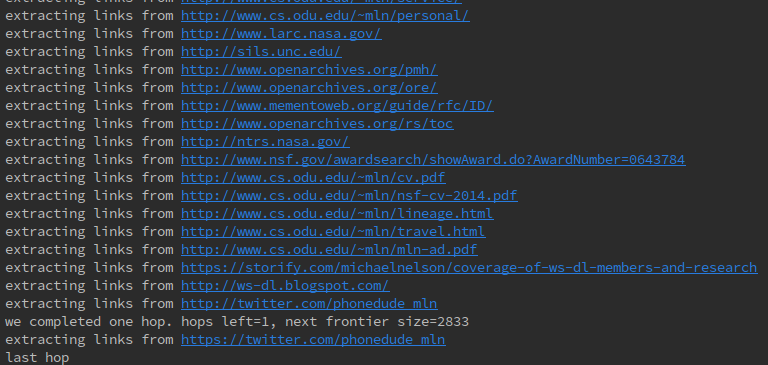
\includegraphics[scale=0.5]{crawlerOutput.png}
\caption{Frontier Size}
\label{fig:frontierSize}
\end{figure}
\begin{code}
\pycode{code/crawler.py}
\captionof{listing}{Python Single Threaded Crawler}
\label{code:crawler}
\end{code}
\newpage
\clearpage
\bibliography{refrences}

\end{document}